Για την κίνηση των σωμάτων θεμελιώθηκαν οι κινηματικοί νόμοι από το Νεύτωνα με το έργο του \textlatin{Principia} (\lat{Philosophiæ Naturalis Principia Mathematica}, 1687). Η νευτώνια κινηματική περιγράφει την κίνηση των αντικειμένων σε ένα αδρανειακό, μη κινούμενο δηλαδή, σύστημα αναφοράς. Όταν εξετάζονται κινήσεις μεγάλης κλίμακας, τέτοιας ώστε η περιστροφή της γης γύρω από τον άξονά της να τις επηρεάζει, η νευτώνια κινηματική δεν μπορεί να τις περιγράψει πλήρως.

Στις εξισώσεις κίνησης ενός σώματος, το οποίο κινείται σε σχέση με ένα περιστρεφόμενο σύστημα αναφοράς, σαν αυτό της περιστρεφόμενης γης, εμφανίζεται μία φαινόμενη δύναμη, η δύναμη \cor. Η δύναμη αυτή πήρε το όνομά της από το Γάλλο επιστήμονα  Γκασπάρ - Γκoυστάβ ντε Κοριόλις (γαλλ. \lat{Gaspard-Gustave de Coriolis}).

Η επιρροή του περιστρεφόμενου συστήματος στην κίνηση του σώματος μπορεί να προσδιοριστεί υπολογίζοντας τον αριθμό \textit{\ros}
\begin{equation}
	Ro = \frac{U}{{Lf}}
\end{equation}
όπου $U$ και $L$ είναι η χαρακτηριστική ταχύτητα και το χαρακτηριστικό μήκος αντίστοιχα, ενώ $f$ η παράμετρος \cor . Ο αριθμός \cor  είναι στην ουσία ο λόγος των αδρανειακών δυνάμεων προς τις δυνάμεις \cor  και είναι χαρακτηριστικός για το σύστημα. Οι δυνάμεις \cor  είναι εμφανείς και ισχυρές και υπερισχύουν των αδρανειακών δυνάμεων, όταν ο αριθμός \ros είναι μικρός. Το σύστημα επέρχεται σε ισορροπία με τη δράση της δύναμης \cor  και της βαθμίδας πίεσης. Η ισορροπία αυτή ονομάζεται \textit{γεωστροφική ισορροπία}. Αντίθετα, όταν ο αριθμός \ros είναι μεγάλος, οι αδρανειακές δυνάμεις υπερισχύουν και το σύστημα έρχεται σε ισορροπία υπό την επίδραση της κεντρομόλου και της φυγόκεντρου δύναμης, όπως ονομάζεται \textit{κυκλοστροφική ισορροπία} (Χαλδούπης, 2015).

\subsection{Παράμετρος \cor \lat{f}}	
Η παράμετρος \cor, γνωστή και ως συχνότητα \cor, εξαρτάται από την ταχύτητα περιστροφής της γης $Ω$ και το γεωγραφικό πλάτος $φ$ εξέλιξης του φαινομένου. Η καμπυλότητα της επιφάνειας της γης μπορεί να αγνοηθεί για αποστάσεις μικρότερες των 100 \lat{km}. Έτσι, τοποθετώντας το σύστημα συντεταγμένων στην επιφάνεια της θάλασσας, με τον άξονα $z$ κατακόρυφα σε αυτή, η παράμετρος \cor \lat{f} μπορεί να θεωρηθεί σταθερή. Η τιμή της παραμέτρου υπολογίζεται ως
\begin{equation}
	f=2Ωsinφ
\end{equation}
Η τιμή αλλάζει πρόσημο κατά τη μετάβαση από το βόρειο προς το νότιο ημισφαίριο, και αντίθετα, ενώ γίνεται 0 στον ισημερινό.

Το όνομα συχνότητα \cor προήλθε από τις αδρανειακές ταλαντώσεις, που έχουν συχνότητα ίση με την παράμετρο \cor. Οι ταλαντώσεις αυτές ονομάζονται και αδρανειακά κύματα. Τα κύματα αυτά είναι εγκάρσια και παρατηρούνται τόσο στην ατμόσφαιρα (πχ. \textit{γεωστροφικός άνεμος}), όσο και στους ωκεανούς και στις λίμνες (\textit{γεωστροφικά ρεύματα}). Τα κύματα τα οποία επηρεάζονται από την κλίση του πυθμένα ονομάζονται κύματα \ros.

\subsection{Μετασχηματισμός θέσης σε περιστρεφόμενο σύστημα αναφοράς}
Θεωρώντας ένα σωματίδιο ακίνητο σε καρτεσιανό αδρανειακό σύστημα αναφοράς, η θέση του περιγράφεται από το διάνυσμα $\bm{X}=e_1x_1+e_2x_2+e_3x_3$. Σε μητρωική μορφή, το διάνυσμα θέσης στο αδρανειακό σύστημα είναι
\begin{equation}
\bm{X}=
\begin{pmatrix}
	e_1 & e_2 & e_3
\end{pmatrix}
\begin{pmatrix}
  x_{1} \\
  x_{2} \\
  x_{3} \\
\end{pmatrix}
\end{equation}

Σε ένα άλλο καρτεσιανό σύστημα, το οποίο έχει περιστραφεί \textit{αριστερόστροφα} σε σχέση με το προηγούμενο κατά μία γωνία $θ$, η θέση του σωματιδίου περιγράφεται από το διάνυσμα 
\begin{equation}
 \label{eq:Xprime}
 \bm{X^{\prime}} =
 \begin{pmatrix}
  x_{1}^{\prime} \\
  x_{2}^{\prime} \\
  x_{3}^{\prime} \\
 \end{pmatrix} = 
 \begin{pmatrix}
  x_{1}cos{θ}+x_{2}sin{θ} \\
  -x_{1}sin{θ}+x_{2}cos{θ} \\
  x_{3} \\
 \end{pmatrix}
\end{equation}
Παρατηρώντας την (\ref{eq:Xprime}), μπορεί να εκλεχθεί ένα μητρώο μετασχηματισμού $\mathbb{R}$ και η θέση του σωματιδίου να περιγράφεται από το διάνυσμα $\bm{X^{\prime}}=\mathbb{E}\mathbb{R}\mathbb{X}$. Το μητρώο αυτό είναι
\begin{equation}
 \label{eq:Rvector}
 \mathbb{R} =
 \begin{pmatrix}
  cos{θ} & sin{θ} & 0 \\
  sin{θ} & cos{θ} & 0 \\
  0      &   0    & 1 \\
 \end{pmatrix}
\end{equation}

\subsection{Περιγραφή του αλγορίθμου}
Η διαδικασία του μετασχηματισμού της θέσης ενός σωματιδίου, που περιγράφηκε παραπάνω, είναι εύκολο να γίνει αλγοριθμικά. Πρέπει να σημειωθεί ότι η διαδικασία αυτή μπορεί να περιγράψει κάθε είδους κίνηση επί του αδρανειακού επιπέδου, καθώς το μόνο απαραίτητο στοιχείο είναι οι καρτεσιανές συντεταγμένες της θέσης του σωματιδίου, οποιαδήποτε στιγμή. Στην κατάστρωση του αλγορίθμου επιλέχθηκε το σώμα να βάλλεται με μία αρχική ταχύτητα $(u, v)$, αντίστοιχα σε κάθε άξονα και έπειτα να ακολουθεί την ευθύγραμμη ομαλή κίνηση. Ακόμα επιλέχθηκε το περιστρεφόμενο σύστημα να περιστρέφεται με σταθερή γωνιακή ταχύτητα, παρόλο που η διαδικασία μπορεί να εφαρμοστεί σε κάθε περίπτωση. Ο λόγος που έγιναν αυτές οι παραδοχές είναι ώστε ο αλγόριθμος να περιγράφει και να αναλύει την κίνηση ενός σωματιδίου στο επίπεδο της γης, καθώς αυτή περιστρέφεται γύρω από τον άξονα της.

'Οπως είναι γνωστό από τη φυσική η θέση ενός σωματιδίου κάθε χρονική στιγμή $i$ δίνεται αναδρομικά από την προηγούμενη
\begin{align}
x_{i} &= x_{i-1}+u\Delta t \\
y_{i} &= y_{i-1}+v\Delta t
\end{align}
όπου $Δt$ είναι ένα απειροστό διάστημα χρόνου και $(u, v)$ οι ταχύτητες σε κάθε άξονα.

Έτσι γνωρίζοντας τη θέση του σωματιδίου στο αδρανειακό σύστημα και ακολουθώντας το μετασχηματισμό (\ref{eq:Xprime}) γίνεται ο υπολογισμός της θέσης του στο περιστρεφόμενο σύστημα. O αλγορίθμου, ο οποίος επιστρέφει τις συντεταγμένες κάθε σημείου της τροχιάς που εκτελεί το σωματίδιο, όπως αυτή αποτυπώνεται στο περιστρεφόμενο σύστημα αναφοράς φαίνεται παρακάτω (βλ. Πίνακα \ref{tab:algCoriolis}).
\begin{table}[h]
	\caption{Αλγόριθμος τροχιάς σημείου σε περιστρεφόμενο σύστημα αναφοράς.}
	\label{tab:algCoriolis}
	\selectlanguage{english}
	\begin{Verbatim}
	\textcolor{green}{ΑΡΧΗ}
	    x0 \textcolor{blue}{=} αρχική θέση στον άξονα x
	    y0 \textcolor{blue}{=} αρχική θέση στον άξονα y
	    θ  \textcolor{blue}{=} 0
	    \textcolor{red}{Για} t \textcolor{blue}{=} 1 \textcolor{red}{έως} t \textcolor{blue}{=} t_Τελικό \textcolor{red}{με_βήμα =} Δt:
	        θ \textcolor{blue}{=} θ \textcolor{blue}{+} Ω \textcolor{blue}{*} Δt
	        x1 \textcolor{blue}{=} x0 \textcolor{blue}{+} u*Δt
	        y1 \textcolor{blue}{=} y0 \textcolor{blue}{+} v*Δt
	        xprime1 \textcolor{blue}{=}  x1*cos(θ) \textcolor{blue}{+} y1*sin(θ)
	        yprime1 \textcolor{blue}{=} \textcolor{blue}{-}x1*sin(θ) \textcolor{blue}{+} y1*cos(θ)
	        τύπωσε(xprime, yprime)
	        x0 \textcolor{blue}{=} x1
	        y0 \textcolor{blue}{=} y1
	    \textcolor{red}{τέλος Για}
	\textcolor{green}{ΤΕΛΟΣ}
	\end{Verbatim}
\end{table}
\newpage

\subsection{Δημιουργία λογισμικού}
Για τη δημιουργία ενός απλού λογισμικού με γραφική διεπαφή χρήστη (\lat{GUI}) έγινε χρήση της γλώσσας προγραμματισμού \lat{Python}. Μέσω της γραφικής διεπαφής ο χρήστης έχει τη δυνατότητα να παράξει γραφικές παραστάσεις της τροχιάς του σωματιδίου, έχοντας παράλληλα πλήρη έλεγχο επί των παραμέτρων. Ο κώδικας που υλοποιεί τον υπολογισμό παρατίθεται στο παράρτημα \ref{sec:corPython}.
\subsubsection{Κυρίως παράθυρο}
\begin{figure}
\centering
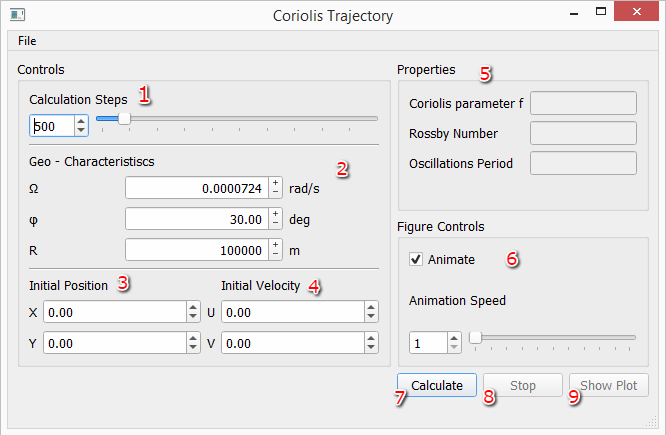
\includegraphics[scale=0.8]{coriolis-gui}
\caption{Γραφική διεπαφή χρήστη του λογισμικού \lat{"Coriolis Trajectory"}.}
\label{fig:coriolis-gui}
\end{figure}
Στο σχήμα \ref{fig:coriolis-gui} φαίνεται το κύριο παράθυρο του λογισμικού. Στην αριστερή μεριά του παραθύρου ο χρήστης έχει τη δυνατότητα να παραμετροποιήσει τη λύση, ενώ στη δεξιά πλευρά εμφανίζονται μερικές χρήσιμες χαρακτηριστικές τιμές καθώς και οι λειτουργίες ελέγχου των παραγώμενων γραφημάτων. Κατά σειρά αρίθμησης
\begin{enumerate}
\item Ορισμός του αριθμού βημάτων επίλυσης
\item Χαρακτηριστικά που αφορούν το επίπεδο επίλυσης
	\begin{itemize}
	\item [\textbf{Ω}] O ρυθμός περιστροφής του επιπέδου, $7.24e^{-5} rad/s$ για το ρυθμό περιστροφής της γης γύρω από τον άξονά της
	\item [\textbf{φ}] Το γεωγραφικό πλάτος εξέλιξης του φαινομένου. Επιτρέπονται τιμές από $-90\degree$ έως $90\degree$. Για τα σωματίδια που εκτελούν κίνηση στον ισημερινό, δηλαδή για $φ=90\degree$ δεν ορίζεται η δύναμη \cor και το πρόγραμμα ειδοποιεί το χρήστη με σχετικό μήνυμα. Ανάλογα με το πρόσημο $\pm$ του γεωγραφικού πλάτους, στο βόρειο ή νότιο ημισφαίριο, το λογισμικό επιλέγει αυτόματα το πρόσημο της γωνιακής ταχύτητας, έτσι ώστε τα αποτελέσματα να έχουν και φυσική υπόσταση.
	\item[\textbf{\lat{R}}] Η ακτίνα του περιστρεφόμενου δακτυλίου. Προτείνεται να μην ξεπερνάει τα 100\lat{km}, καθώς αυτή είναι η οριακή τιμή για την οποία μπορούμε να θεωρήσουμε σταθερή τη συχνότητα \cor \lat{f}.
	\end{itemize}
\item Αρχική θέση του σωματιδίου
\item Αρχική ταχύτητα του σωματιδίου, στις συνιστώσες $(u, v)$ του καρτεσιανού επιπέδου
\item Χαρακτηριστικά της κίνησης
	\begin{description}[style=nextline]
	\item[\small\textbf{Παράμετρος \cor \lat{f}}] Η συχνότητα \cor
	\item[\small\textbf{Αριθμός \ros}] Ο αριθμός \ros, χαρακτηριστικός του φαινομένου.
	\item[\small\textbf{Συχνότητα αδρανειακών ταλαντώσεων}] Η συχνότητα της ταλάντωσης που εκτελεί ένα σωματίδιο ρευστού, κατά την οποία οι αδρανειακές δυνάμεις που του ασκούνται εξισορροπούνται πλήρως από τη δύναμη \cor.
	\end{description}
\item Επιλογή για την απεικόνιση των αποτελεσμάτων σε μορφή βίντεο (\lat{animation}).
\item Το βασικό κουμπί εκτέλεσης του προγράμματος. Ελέγχει τα δεδομένα και στο τέλος των υπολογισμών εμφανίζει τη γραφική παράσταση του αποτελέσματος
\item Στην περίπτωση που οι υπολογισμοί διαρκούν πολύ ώρα, δίνεται στο χρήστη δυνατότητα τερματισμού
\item Εμφανίζει τη γραφική παράσταση, σύμφωνα με τις επιλογές του χρήστη στο $(6)$, χωρίς την επανέναρξη του υπολογισμού
\end{enumerate}

Πρέπει να σημειωθεί ότι έχει υλοποιηθεί προγραμματισμός που κάνει χρήση παραπάνω τους ενός πυρήνα του επεξεργαστή, δίνοντας στο χρήστη τη δυνατότητα να υπολογίσει και να εμφανίσει ταυτόχρονα πολλά διαφορετικά σενάρια επίλυσης.

\subsubsection{Παράθυρο γραφικής παράστασης}
\begin{figure}
\label{fig:cor-graph}
\centering
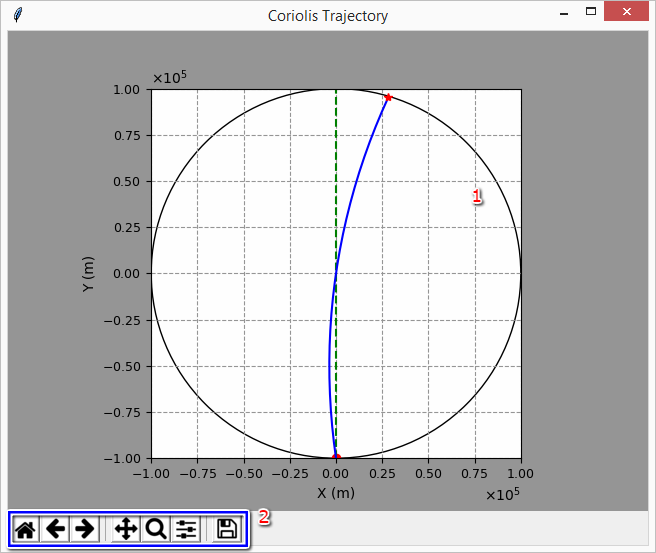
\includegraphics[scale=0.7]{cor-graph}
\caption{Παράθυρο γραφικής παράστασης του λογισμικού \lat{"Coriolis Trajectory"}}
\end{figure}
Το δεύτερο παράθυρο του λογισμικού εμφανίζει γραφικά τα αποτελέσματα των υπολογισμών. Τα αποτελέσματα εμφανίζονται είτε με τη μορφή βίντεο, είτε σταθερά, αναλόγως με την επιλογή του χρήστη. Ακόμα, υπάρχει η δυνατότητα εξαγωγής και αποθήκευσης του γραφήματος σε ένα αρχείο εικόνας. Στο παράθυρο φαίνονται
\begin{enumerate}
\item Το κυρίως γράφημα
\begin{description}[style=nextline]
\item[\small{Μαύρη γραμμή}] Τα όρια του περιστρεφόμενου κυκλικού δίσκου
\item[\small{Πράσινη γραμμή}] Η τροχιά του σωματιδίου στο αδρανειακό σύστημα αναφοράς
\item[\small{Μπλε γραμμή}] Η τροχιά του σωματιδίου στο περιστρεφόμενο σύστημα αναφοράς
\item[\small{Κόκκινος κύκλος}] Η αρχική θέση του σωματιδίου
\item[\small{Κόκκινο αστέρι}] Η τελική θέση του σωματιδίου
\end{description}
\item Επιλογές για την παραμετροποίηση της εμφάνισης του γραφήματος, καθώς και αποθήκευσής του σε αρχείο εικόνας
\end{enumerate}

\subsection{Αποτελέσματα και Σχολιασμός}
Το λογισμικό επιστρέφει στο χρήστη μερικές χρήσιμες τιμές, ώστε αυτός να μπορεί να αξιολογήσει τα αποτελέσματα. Μία από αυτές είναι ο αριθμός \ros. Ο αριθμός αυτός αποτελεί τον αδιάστατο λόγο των αδρανειακών δυνάμεων προς τις δυνάμεις \lat{Coriolis}. 

Η τάξη μεγέθους αυτού του αριθμού δηλώνει κατά πόσο η τροχιά ενός σωματιδίου επηρεάζεται από την περιστροφή του συστήματος συντεταγμένων, όπως για παράδειγμα όταν ένα σωματιδίου που εκτελεί μία κίνηση επηρεάζεται από την περιστροφή της γης γύρω από τον άξονα της. Όταν η τιμή του αριθμού \lat{Rossby} είναι αρκετά μεγάλη, δηλαδή οι αδρανειακές δυνάμεις υπερισχύουν των δυνάμεων \lat{Coriolis} και το σύστημα έρχεται σε κυκλοστροφική ισορροπία, φαίνεται ότι η τροχιά του σωματιδίου δεν επηρεάζεται από την περιστροφή του συστήματος. \textbf{[ΑΝΑΦΟΡΑ ΕΙΚΟΝΑΣ ΕΔΩ]}. Στην αντίθετη περίπτωση που ο αριθμός \ros είναι μικρός, το σύστημα έρχεται σε γεωστροφική ισορροπία και οι δυνάμεις \cor υπερισχύουν των αδρανειακών δυνάμεων, η τροχιά του σωματιδίου επηρεάζεται σε μεγάλο βαθμό από την περιστροφή του συστήματος συντεταγμένων. \textbf{[ΑΝΑΦΟΡΑ ΕΙΚΟΝΑΣ ΕΔΩ]}

\subsubsection{Αδρανειακές Ταλαντώσεις}
Οι αδρανειακές ταλαντώσεις είναι η πιο απλή μορφή κίνησης στη γη, η οποία επηρεάζεται από τη χρονική της διάρκεια. Στην πραγματικότητα, τέτοιου είδους κίνηση δεν εμφανίζεται μόνο στην περίπτωση της περιστρεφόμενης γης. Ένα απλό παράδειγμα για την κατανόηση των δυνάμεων που επηρεάζουν τέτοιες κινήσεις, είναι το παράδειγμα του περιστρεφόμενου παραβολικού δίσκου.
\begin{figure}[ht]
	\centering
	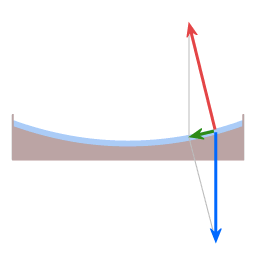
\includegraphics[scale=0.7]{images/coriolis-parabolic-disk.png}
	\caption{Οι δυνάμεις στο πείραμα του περιστρεφόμενου παραβολικού δίσκου. \lat{\cite{parbolicDisk}}}
	\label{fig:coriolis-parbolic-disk}
\end{figure}

Στο πείραμα του περιστρεφόμενου παραβολικού δίσκου, Σχήμα \ref{fig:coriolis-parbolic-disk}, αφήνεται ένα σώμα να εκτελέσει μία ελεύθερη ταλάντωση στην άτριβη επιφάνεια. Η δύναμη επαναφοράς είναι ανάλογη της απόστασης από το κέντρο της παραβολής. Παρατηρώντας αυτήν την κίνηση από ένα αδρανειακό σύστημα, φαίνεται ότι το σώμα εκτελεί μία ελλειπτική κίνηση, η οποία ονομάζεται αδρανειακή ταλάντωση.

Στο φυσικό κόσμο, η δύναμη επαναφοράς είναι η φαινόμενη δύναμη \lat{Coriolis}. Η περιστροφή της γης επηρεάζει τις κινήσεις που είναι πολύ "αργές" σε σχέση με την περιστροφή της, όπως τα κύματα με μεγάλο μήκος και μικρή συχνότητα, τα αδρανειακά κύματα (\lat{inertial waves}).

Τα αδρανειακά κύματα είναι εγκάρσια μηχανικά κύματα, που σε αντίθεση με τα επιφανειακά, λαμβάνουν χώρα στα εσωτερικά στρώματα ενός ρευστού. Τέτοια κύματα εμφανίζονται συνήθως στην ατμόσφαιρα της γης, παραδείγματος χάρη τα κύματα \lat{Rossby} και τα γεωστροφικά ρεύματα.

Τέτοια κύματα συναντώνται και στον ωκεανό, με τη μορφή κυμάτων \lat{Poincare}. Κύμα \lat{Poincare} μπορεί να θεωρηθεί και η διάδοση της παλίρροιας, καθώς και όλα τα κύματα ρηχού στρώματος (\lat{SWW}), μακριά από τη στεριά.

Η συχνότητα των επιφανειακών κυμάτων \lat{Poincare} είναι ίδια με την συχνότητα κυμάτων ρηχού στρώματος, με την προσθήκη της παραμέτρου \lat{Coriolis}, \lat{f}.
\begin{equation}
	ω = \sqrt{f^2+gHk^2}
\end{equation}

Η ταχύτητα ομάδας (\lat{Group velocity}) είναι
\begin{equation}
	C_g = \dfrac{\partial{ω}}{\partial{k}} = \dfrac{gHk}{\sqrt{f^2+gHk^2}}
\end{equation}

Όταν $f \rightarrow 0$ ή $k^2 \gg \dfrac{f^2}{gH}$ τότε $C_g=\sqrt{gH}$ και το κύμα συμπεριφέρεται σαν απλό κύμα ρηχού στρώματος, χωρίς της επιρροή της περιστροφής της γης. Στην αντίθετη περίπτωση, όπου $k \rightarrow 0$ τότε $C_g = 0$, δεν υπάρχει διάδοση του κύματος και εκτελείται μία αδρανειακή ταλάντωση.

Η επίλυση στη μία διάσταση ενός κύματος \lat{Poincare} είναι
\begin{align}
	u &= \dfrac{ω}{kH}H_0\cos(kx-ωt) \\
	v &= \dfrac{f}{kH}H_0\sin(kx-ωt)
\end{align}

Εύκολα, μπορούμε να υπολογίσουμε πότε η περιστροφή της γης είναι σημαντική. Η χαρακτηριστική κλίμακα μήκους είναι
\begin{equation}
	L \rightarrow 1/k \Rightarrow L_R = \dfrac{\sqrt{gH}}{H}
\end{equation}
και ονομάζεται \textbf{\lat{Rossby radius of deformation}}. Για μήκος μικρότερο από την τιμή της κλίμακας η περιστροφή δεν επηρεάζει την κίνηση.

\subsubsection{Υπολογισμός του αριθμού \ros}
Ο αριθμός \ros αποτελεί έναν αδιάστατο αριθμό χαρακτηριστικό για το κάθε πρόβλημα, ο δε υπολογισμός του είναι εύκολος κάνοντας χρήση και ανάλυση των εγγενών κλιμάκων του προβλήματος.

Έχοντας ως βασική κλίμακα το \textbf{χρόνο}, μπορεί να προσδιοριστεί τόσο ο χρόνος που απαιτείται ώστε ένα σημείο επάνω στο όριο του κύκλου που περιγράφει το περιστρεφόμενο σύστημα αναφοράς να κάνει μία πλήρη περιστροφή, όσο και ο χρόνος που απαιτείται ώστε ένα σωματίδιο, που εκτελεί την εξεταζόμενη κίνηση, να διαγράψει μία διαμετρική πορεία.

Ο χρόνος που απαιτείται ώστε ένα σημείο του κύκλου να διαγράψει μία πλήρη περιστροφή είναι
\begin{equation}
\label{eq:t_r}
t_{R}=\frac{2\pi}{\Omega}
\end{equation}
ενώ ο χρόνος που απαιτείται ώστε ένα σωματίδιο να εκτελέσει ευθύγραμμη ομαλή κίνηση και να διαγράψει απόσταση ίση με τη διάμετρο του κυκλικού δίσκου είναι
\begin{equation}
\label{eq:t_i}
t_{I}=\frac{2R}{\mathbb{V}}
\end{equation}
όπου $Ω$ είναι η σταθερή γωνιακή ταχύτητα του κυκλικού δίσκου, $R$ η διάμετρός του και $\mathbb{V}$ η χαρακτηριστική ταχύτητα της ευθύγραμμης κίνησης.

Συνδυάζοντας τις \ref{eq:t_r} και \ref{eq:t_i}, που έχουν ως κλίμακα το χρόνο, $[T]$, προκύπτει ο αδιάστατος αριθμός \ros
\begin{equation}
\label{eq:ro}
Ro = \dfrac{t_{R}}{t_{I}} \; \Rightarrow \;
Ro = \dfrac{\dfrac{2π}{Ω}}{\dfrac{2R}{\mathbb{V}}}
\end{equation}

Κάνοντας τις απλοποιήσεις και απαλοίφοντας το σταθερό όρο $π$, προκύπτει ο αριθμός \ros που χρησιμοποιήθηκε στο λογισμικό
\begin{equation}
Ro = \dfrac{\mathbb{V}}{ΩR}
\end{equation}